% Options for packages loaded elsewhere
\PassOptionsToPackage{unicode}{hyperref}
\PassOptionsToPackage{hyphens}{url}
%
\documentclass[
]{article}
\usepackage{amsmath,amssymb}
\usepackage{iftex}
\ifPDFTeX
  \usepackage[T1]{fontenc}
  \usepackage[utf8]{inputenc}
  \usepackage{textcomp} % provide euro and other symbols
\else % if luatex or xetex
  \usepackage{unicode-math} % this also loads fontspec
  \defaultfontfeatures{Scale=MatchLowercase}
  \defaultfontfeatures[\rmfamily]{Ligatures=TeX,Scale=1}
\fi
\usepackage{lmodern}
\ifPDFTeX\else
  % xetex/luatex font selection
\fi
% Use upquote if available, for straight quotes in verbatim environments
\IfFileExists{upquote.sty}{\usepackage{upquote}}{}
\IfFileExists{microtype.sty}{% use microtype if available
  \usepackage[]{microtype}
  \UseMicrotypeSet[protrusion]{basicmath} % disable protrusion for tt fonts
}{}
\makeatletter
\@ifundefined{KOMAClassName}{% if non-KOMA class
  \IfFileExists{parskip.sty}{%
    \usepackage{parskip}
  }{% else
    \setlength{\parindent}{0pt}
    \setlength{\parskip}{6pt plus 2pt minus 1pt}}
}{% if KOMA class
  \KOMAoptions{parskip=half}}
\makeatother
\usepackage{xcolor}
\usepackage[margin=1in]{geometry}
\usepackage{graphicx}
\makeatletter
\def\maxwidth{\ifdim\Gin@nat@width>\linewidth\linewidth\else\Gin@nat@width\fi}
\def\maxheight{\ifdim\Gin@nat@height>\textheight\textheight\else\Gin@nat@height\fi}
\makeatother
% Scale images if necessary, so that they will not overflow the page
% margins by default, and it is still possible to overwrite the defaults
% using explicit options in \includegraphics[width, height, ...]{}
\setkeys{Gin}{width=\maxwidth,height=\maxheight,keepaspectratio}
% Set default figure placement to htbp
\makeatletter
\def\fps@figure{htbp}
\makeatother
\setlength{\emergencystretch}{3em} % prevent overfull lines
\providecommand{\tightlist}{%
  \setlength{\itemsep}{0pt}\setlength{\parskip}{0pt}}
\setcounter{secnumdepth}{-\maxdimen} % remove section numbering

\newcommand{\beginsupplement}{%
        \setcounter{table}{0}
        \renewcommand{\thetable}{S\arabic{table}}%
        \setcounter{figure}{0}
        \renewcommand{\thefigure}{S\arabic{figure}}%
     }

\usepackage{lineno}
\linenumbers

\usepackage{natbib}

\usepackage{setspace} \doublespacing
\ifLuaTeX
  \usepackage{selnolig}  % disable illegal ligatures
\fi
\IfFileExists{bookmark.sty}{\usepackage{bookmark}}{\usepackage{hyperref}}
\IfFileExists{xurl.sty}{\usepackage{xurl}}{} % add URL line breaks if available
\urlstyle{same}
\hypersetup{
  pdftitle={Transcripts with high distal heritability mediate genetic effects on complex traits},
  hidelinks,
  pdfcreator={LaTeX via pandoc}}

\title{Transcripts with high distal heritability mediate genetic effects
on complex traits}
\author{}
\date{\vspace{-2.5em}}

\begin{document}
\maketitle

\subsection{Abstract}\label{abstract}

The transcriptome is increasingly viewed as a bridge between genetic
risk factors for complex disease and their associated pathophysiology.
Powerful insights into disease mechanism can be made by linking genetic
variants affecting gene expression (expression quantiatitive trait loci
- eQTLs) to phenotypes.

\subsection{Introduction}\label{introduction}

In the quest to understand genetic contributions to complex traits, gene
expression is an important bridge between genotype and phenotype. The
majority of variants identified in GWAS are in regulatory regions of the
genome {[}cite{]}, suggesting that they influence clinical phenotypes
through regulation of gene expression. Consistent with this idea,
powerful insights into disease mechanism can be made by linking genetic
variants affecting gene expression (expression quantitative trait loci -
eQTLs) to phenotypes. In particular, mediation analysis has been used to
identify transcripts that mediate the effect of genetic variants on
phenotypes. In mice\ldots{}
\cite{pmid29567659,pmid31465442,pmid35672473} (bmediatR)
\cite{pmid35533209} In humans\ldots{} \cite{pmid25533967,pmid24232670}

Thus far, the primary focus of expression mediated traits has been on
local genetic variation; that is genetic variation that influences the
transcription of local genes, thereby causing variation in traits.
However, there is evidence that the bulk of disease heritability is
mediated by the distal component of gene expression, rather than the
local component \cite{pmid32424349}. Yao et al.~{[}cite{]} observed that
genes with low local heritability explain more expression-mediated
disease heritability than genes with high local heritability. We have
observed a similar pattern in mice, which we describe here. Thus,
identifying heritable components of complex traits that are mediated
through distally regulated variation in gene expression may provide
important insights into mechanisms regulating complex traits.

Identification of distal factors influencing gene expression and traits
is challenging, as the multiple testing corrections are much more severe
for distal effects \cite{pmid24013639}. However, systems approaches that
consider the entire transcriptome simultaneously and avoid univariate
testing provide promising avenues for identification of broad
transcriptomic patterns influencing complex traits that provide both
biological insight and targets for therapeutics. Here we propose
high-dimenaional mediation (HDM) as one such systems approach for
identification of the heritable portion of the transcriptome that
mediates the effect of the genome on phenome. HDM uses a regularized and
generalized canonical correlation analysis (RGCCA) {[}cite{]}, which is
an extension of canonical correlation analysis (CCA) that allows for
more than two data sets with an arbitrary relationship among them. Thus,
we can identify linear combinations of the genome, transcriptome, and
phenome, that describe the mediation of the genetic effects on the
phenome through the transcriptome. Because of the central dogma of
molecular biology, information flow is directed out of the genome, and
not back into it. Thus, the otherwise undirected relationships between
genome, transcriptome, and phenome can be inferred as a causal mediation
by the transcriptome of the effects of the genome on the phenome.

Here we apply HDM

\subsection{Results}\label{results}

\subsubsection{Genetic variation contributes to wide phenotypic
variation}\label{genetic-variation-contributes-to-wide-phenotypic-variation}

A population of 500 diversity outbred mice (XXX male and XXX female),
was placed on a high-fat (XXX/\%), high-sugar (XXX/\%) diet starting at
XXX weeks of age as described previously {[}cite{]}. Each individual was
assessed longitudinally for multiple metabolic measures including
fasting glucose levels, glucose tolerance, insulin levels, body weight,
and blood lipid levels (Methods).

Although the environment was consistent across animals, the genetic
diversity present in this population resulted in widely varying
distributions across physiological measurements (Fig.
\ref{fig:trait_overview}). For example, body weights of adult
individuals varied from less than the average adult B6 body weight to
several times the body weight of a B6 adult in both sexes (Fig.
\ref{fig:trait_overview}A). Fasting blood glucose also varied
considerably (Fig. \ref{fig:trait_overview}B) although few of the
animals had FBG levels that would indicate pre-diabetes ( animals, ), or
diabetes (7 animals, 1.4) according to previously developed cutoffs
(pre-diabetes: FBG \(\geq\) 250 mg/dL, diabetes: FBG \(\geq\) 300,
mg/dL) \cite{pmid17018838}. Males had higher FBG than females on average
(Fig. \ref{fig:trait_overview}C) as has been observed before suggesting
either that males were more susceptible to metabolic disease on the
high-fat diet, or that males and females may require different
thresholds for pre-diabetes and diabetes.

Body weight was strongly positively correlated with food consumption
(Fig. \ref{fig:trait_overview}D \(R^2 =\) 0.51, \(p=\)
\ensuremath{1.5\times 10^{-75}}) and fasting blood glucose (FBG) (Fig.
\ref{fig:trait_overview}E, \(R^2=\) 0.25, \(p =\)
\ensuremath{2\times 10^{-32}}) suggesting a link between behavioral
factors and metabolic disease. However, the heritability of this trait
and others (Fig. \ref{fig:trait_overview}F) indicates that background
genetics contribute substantially to correlates of metabolic disease in
this population.

\begin{figure}[ht!]
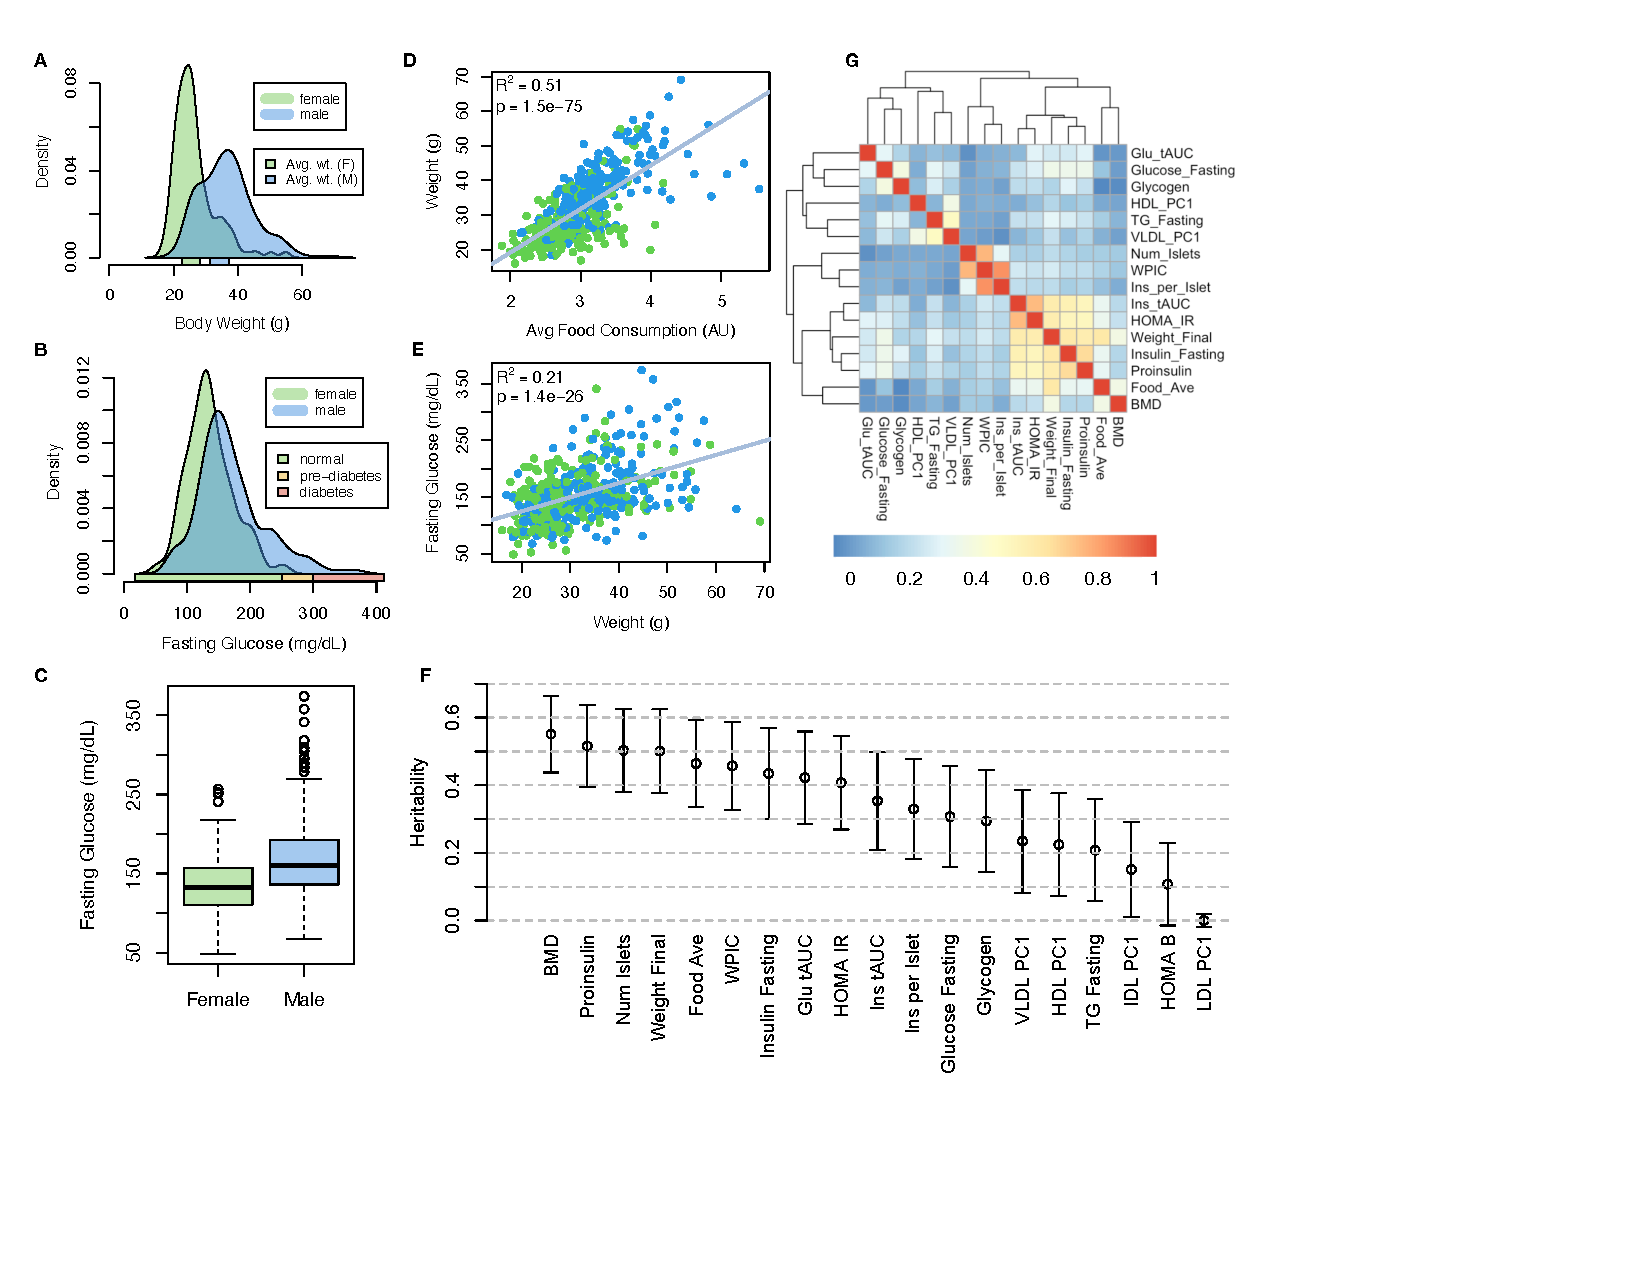
\includegraphics[width=\textwidth]{Figures/Fig1_trait_overview.pdf} 
\caption{Clinical overview. \textbf{A.} Distributions of final body weight 
in the diversity outbred mice. Sex is indicated by color. The 
average B6 male and female adult weights at 24 weeks of age 
are indicated by blue and green bars on the x-axis. \textbf{B.} The 
distribution of final fasting glucose across the population split 
by sex. Normal, pre-diabetic, and diabetic fasting glucose levels 
for mice are shown by colored bars along the x-axis. \textbf{C.} Males had 
higher fasting blood glucose on average than females. \textbf{D.} The 
relationship between food consumption and body weight for both 
sexes. \textbf{E.} Relationship between body weight and fasting glucose 
for both sexes. \textbf{F.} Heritability estimates for each physiological 
trait. Bars show standard error of the estimate. \textbf{G.} Correlation 
structure between pairs of physiological traits.}
\label{fig:trait_overview}
\end{figure}

The landscape of trait correlations (Fig. \ref{fig:trait_overview}G)
shows that most of the metabolic trait pairs were relatively weakly
correlated indicating complex relationships among the measured traits.
This low level of redundancy suggests a broad sampling of multiple
heritable aspects of metabolic disease including overall body weight,
glucose homeostasis, pancreatic composition and liver function.

\subsubsection{Distal Heritability Correlates with Phenotype
Relevance}\label{distal-heritability-correlates-with-phenotype-relevance}

To elaborate the mechanistic details of genetic effects on metabolic
phenotypes in the DO population, we also measured gene expression in
four tissues known to be involved in metabolic disease: adipose,
pancreatic islet, liver, and skeletal muscle. To confirm the
heritability of transcript levels, we performed expression QTL analysis
using R/qtl2 {[}cite{]} (Methods) and identified both local and distal
eQTL for transcripts in each tissue (Supp. Fig \ref{fig:eQTL}).
Significant local eQTLs far outnumbered distal eQTLs (Supp. Fig.
\ref{fig:eQTL}F) and tended to be shared across tissues (Supp. Fig.
\ref{fig:eQTL}G) whereas the few significant distal eQTL we identified
tended to be tissue-specific (Supp. Fig. \ref{fig:eQTL}H)

To better compare the relative contribution of local and distal genetics
to transcript levels, we performed a heritability analysis for each
transcript (Methods). Overall, local and distal factors contributed
approximately equally to transcript abundance. In all tissues, both
local and distal factors explained between 13 and 19\% of the variance
in the median transcript (Fig \ref{fig:motivation}A).

\begin{figure}[ht!]
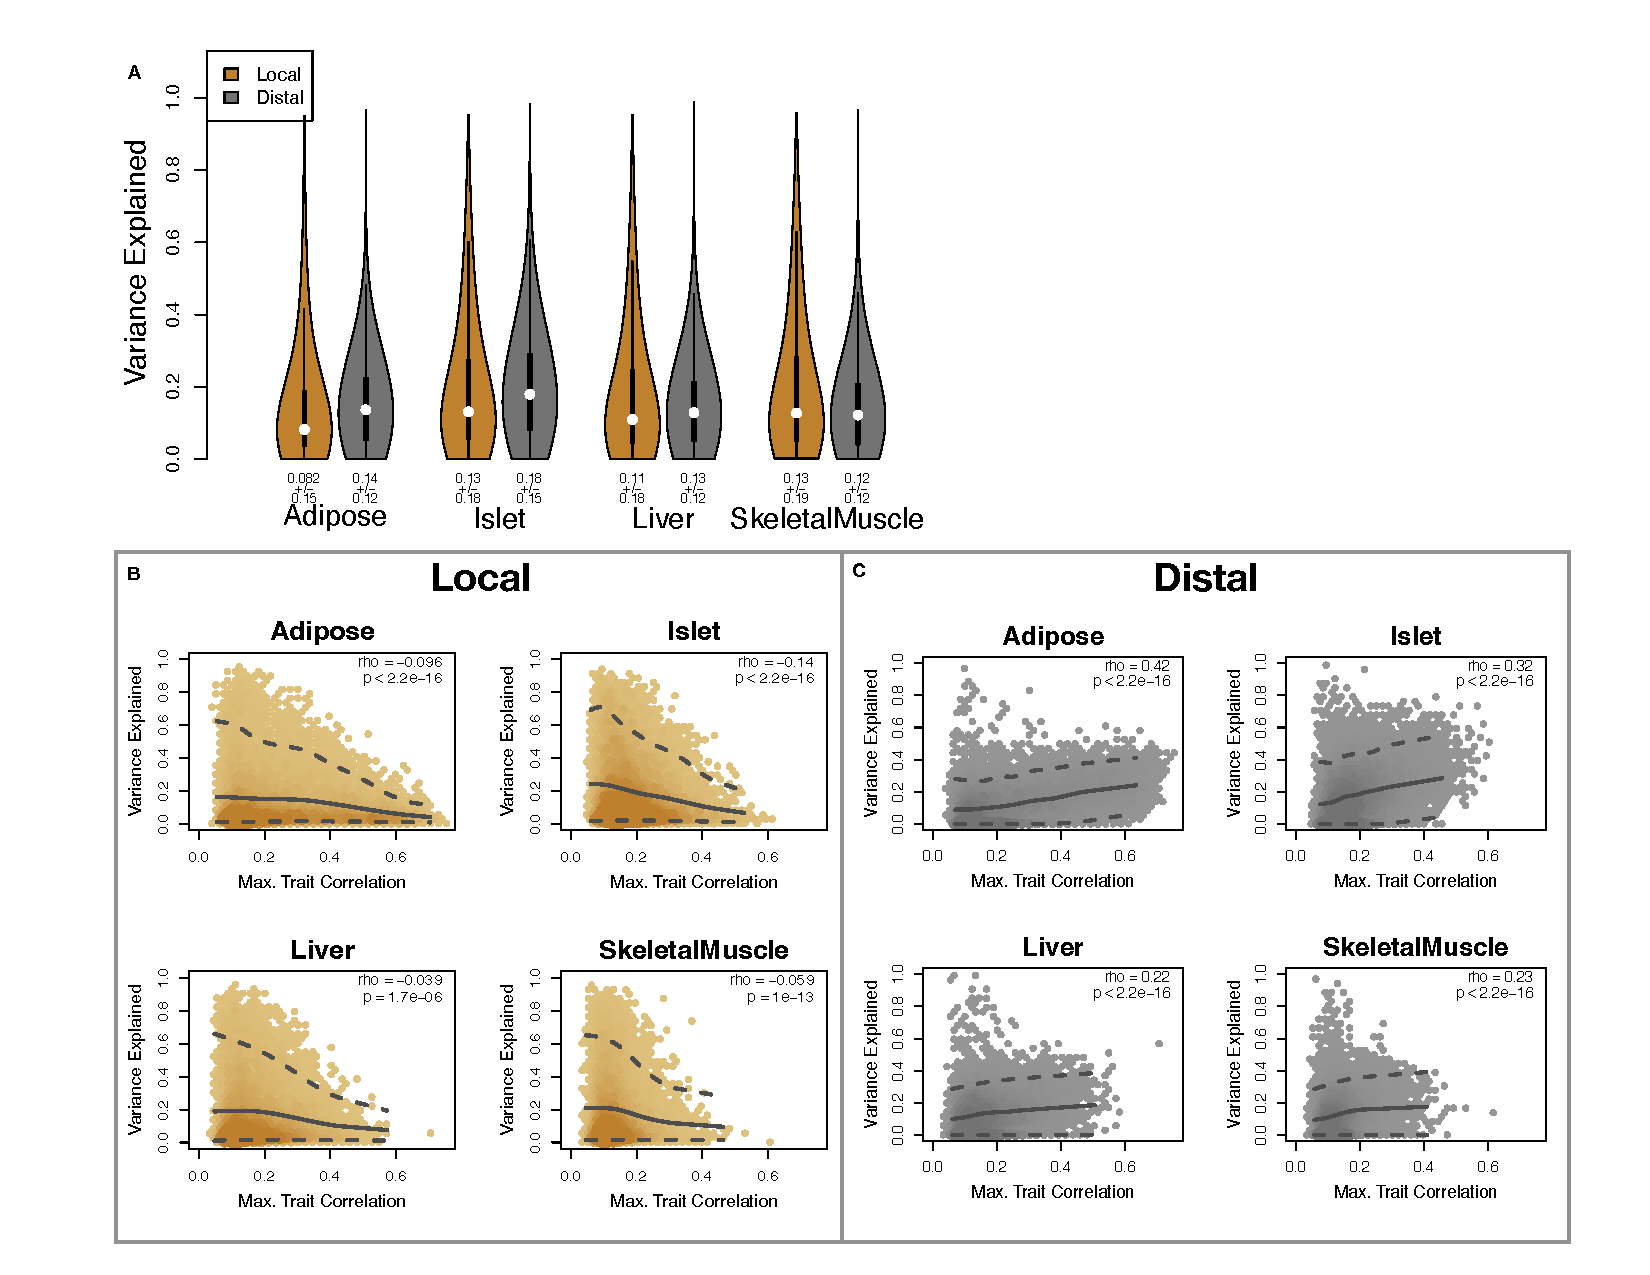
\includegraphics[width=\textwidth]{Figures/Fig2_motivation.pdf} 
\caption{Transcript heritability and trait relevance. 
\textbf{A.} Distributions of distal and local heritability of 
transcripts across the four tissues. Overall local and distal 
factors contribute equally to transcript heritability. The 
relationship between (\textbf{B.}) local and (\textbf{C.}) 
distal heritability and trait relevance across all four tissues. 
Here trait relevance is defined as the maximum correlation between 
the transcript and all traits. Local heritability is negatively 
correlated with trait relevance, and distal heritability is 
positively correlated with trait relevance. Pearson ($r$) and $p$ 
values for each correlation are shown in the upper-right of each panel.}
\label{fig:motivation}
\end{figure}

Local heritability of transcripts was negatively correlated with their
trait relevance, defined as the maximum correlation of a transcript
across all traits (Fig. \ref{fig:motivation}B). This suggests that the
more local genotype influenced transcript abundance, the less effect
variation in transcript abundance was related to the measured traits.
Conversely, distal heritability of transcripts was positively correlated
with trait relevance (Fig. \ref{fig:motivation}C). That is, transcripts
that were more highly correlated with the measured traits tended to be
distally, rather than locally, heritable. That trait-correlated
transcripts have low local heritability is consistent with previous
observations that low-heritability transcripts explain more
expression-mediated disease heritability than high-heritability
transcripts \cite{pmid32424349}. However, the positive relationship
between trait correlation and distal heritability suggests that there
are alternative mechanisms through which genetic regulation of
transcripts may influence traits.

\subsubsection{High-Dimensional Mediation identifies composite
transcript that perfectly mediates composite
trait}\label{high-dimensional-mediation-identifies-composite-transcript-that-perfectly-mediates-composite-trait}

To identify mechanisms through which genetic regulation of transcripts
influences heritable traits, we propose high-dimensional mediation (HDM)
(Fig. \ref{fig:workflow}). In this process we kernelize each of the
genome, transcriptome, and phenome, and perform regularized and sparse
generalized canonical correlation analysis (RGCCA) {[}cite{]} in which
we explicitly model the mediation by the transcriptome of the effect of
the genome on the phenome (Methods, Fig. \ref{fig:workflow}). RGCCA is
an extended form of canonical correlation analysis (CCA) {[}cite{]} in
which multiple data sets can be analyzed simultaneously with explicit
relationships.

\begin{figure}[ht!]
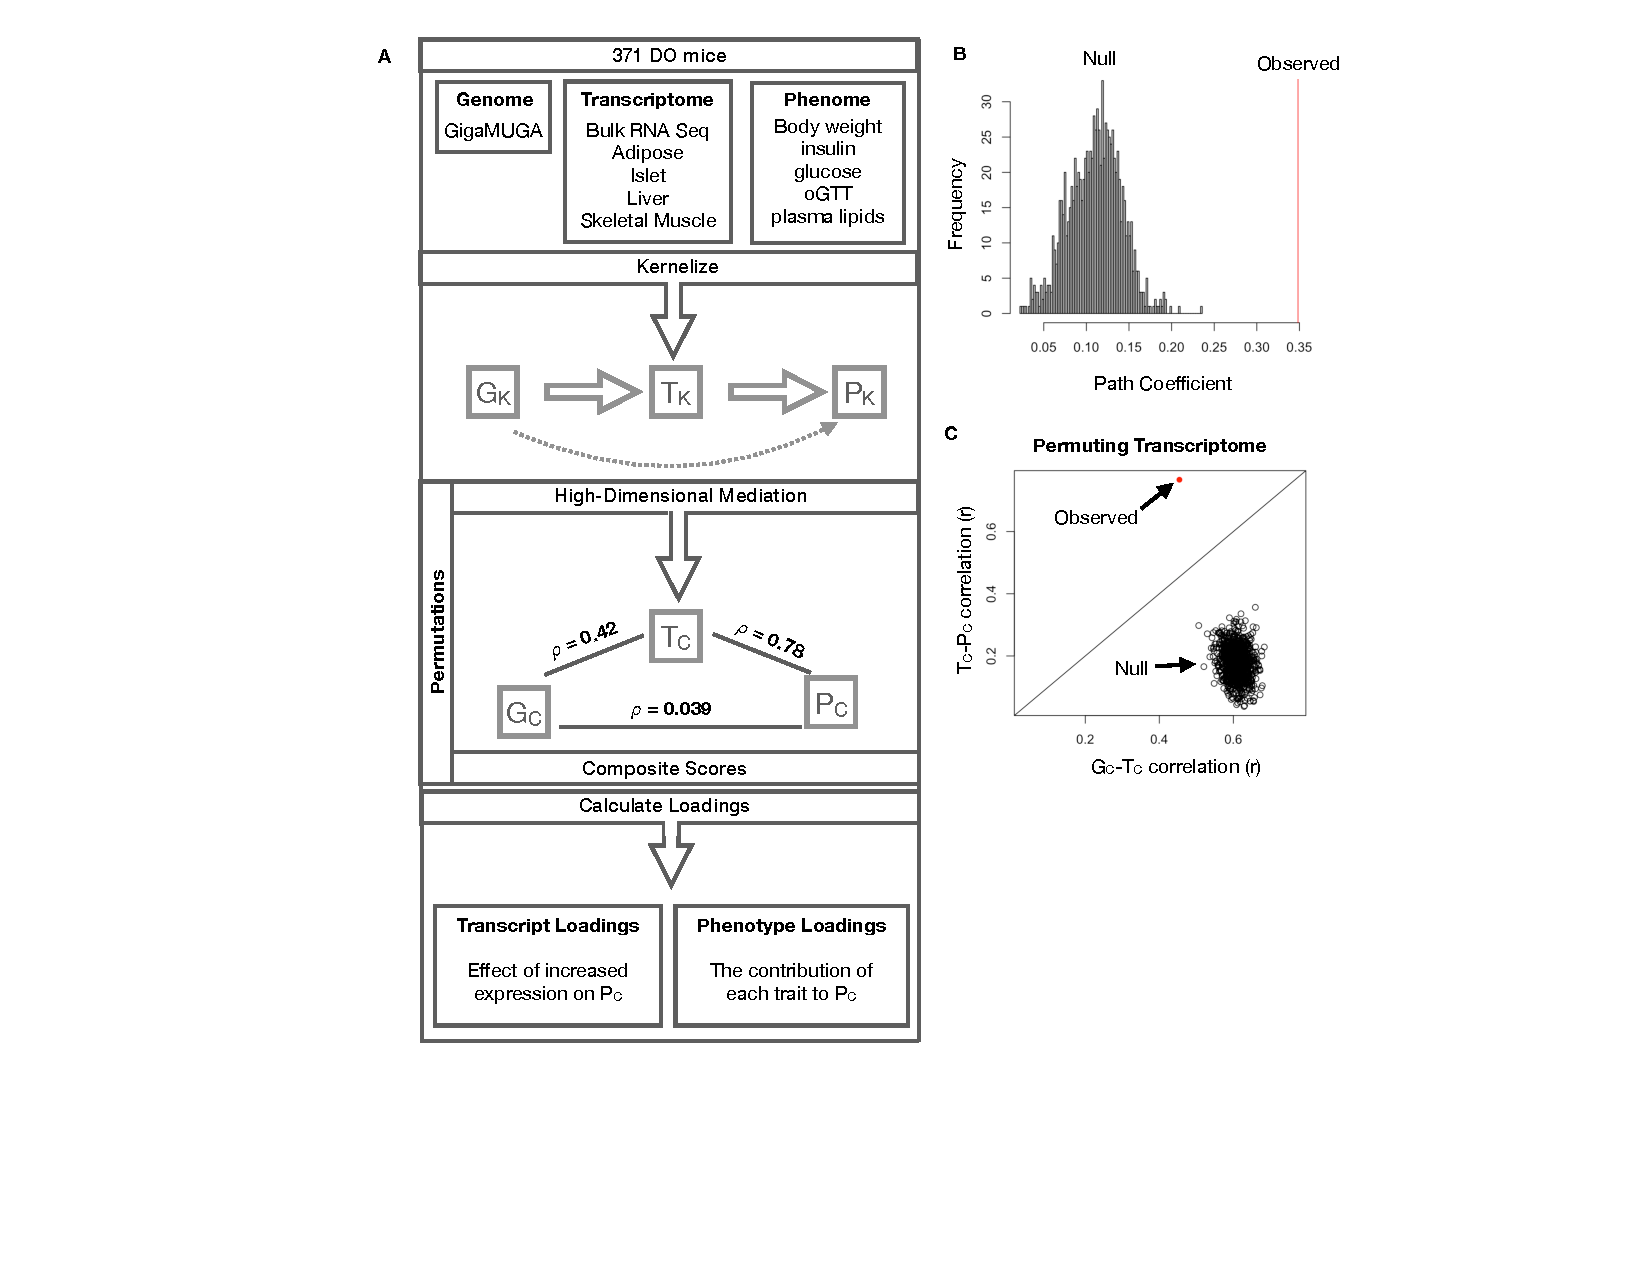
\includegraphics[width=5in]{Figures/Fig3_workflow.pdf} 
\caption{High-dimensional mediation. \textbf{A.} Workflow indicating 
major steps of high-dimensional mediation. The genotype, transcriptome, 
and phenotype matrices were kernelized to yield single matrices representing 
the relationships between all individuals for each data modality ($G_K$ = 
genome kernel, $T_K$ = transcriptome kernel; $P_K$ = phenome kernel). High-dimensional 
mediation was applied to these matrices to maximize the direct path 
$G \rightarrow T \rightarrow P$, the mediating pathway (arrows), while 
simultaneously minimizing the direct $G \rightarrow P$ pathway (dotted line). 
The composite vectors that resulted from high-dimensional mediation were 
$G_c$, $T_C$, and $P_C$. The partial correlations $\rho$ between these vectors 
indicated perfect mediation. Transcript and trait loadings were calculated 
as described in the methods. \textbf{B.} The null distribution of the path 
coefficient derived from 10,000 permutations compared to the observed path 
coefficient (red line). \textbf{C.} The null distribution of the $G_C$-$T_C$ 
correlation vs. the $T_C$-$P_C$ correlation compared with the observed value 
(red dot).
}
\label{fig:workflow}
\end{figure}

The result of this process is three vectors representing the composite
genome (\(G_C\)), composite transcriptome (\(T_C\)) and the composite
phenome (\(P_C\)) where the composite transcriptome perfectly mediates
the effect of the composite genome on the composite phenome. Each vector
is of length \(n\) where \(n\) is the number of individual mice. Fig.
\ref{fig:workflow}A shows the partial correlations between all pairs of
composite vectors. The partial correlation \(r\) between \(G_C\) and
\(T_S\) was 0.46, and the partial correlation between \(T_S\) and
\(P_S\) was 0.78. However, when the transcriptome was taken into
account, the partial correlation between \(G_S\) and \(P_S\) was
effectively 0 (-0.01).

Standard CCA is prone to over-fitting because in any two large matrices
it can be trivial to identify highly correlated composite vectors. To
assess whether RGCCA was similarly prone to over-fitting in a
high-dimensional space, we performed permutation testing. We permuted
the individual labels on the transcriptome kernel matrix 1000 times and
recalculated the path coefficient, which is the partial correlation of
\(G_C\) and \(T_C\) multiplied by the partial correlation of \(T_C\) and
\(P_C\). This represents the path from \(G_C\) to \(P_C\) that is
mediated through \(T_C\). The null distribution of the path coefficient
is shown in Fig. \ref{fig:workflow}B, and the observed path coefficient
from the original data is indicated by the red line. The observed path
coefficient was well outside the null distribution generated by
permutations. Fig. \ref{fig:workflow}C illustrates this observation in
more detail. Although we identified high correlations between \(G_C\)
and \(T_C\), and modest correlations between \(T_C\) and \(P_C\) in the
null data (Fig \ref{fig:workflow}C), these two values could not be
maximized simultaneously. The red dot shows that in the real data both
the \(G_C\)-\(T_C\) correlation and the \(T_C\)-\(P_C\) correlation
could be maximized simultaneously suggesting that that path from
genotype to phenotype through transcriptome is highly non-trivial and
identifiable in this case. These results suggest that these composite
vectors represent genetically determined variation in phenotype that is
mediated through genetically determined variation in transcription.

\subsubsection{Body weight and insulin resistance were highly
represented in the expression-mediated composite
trait}\label{body-weight-and-insulin-resistance-were-highly-represented-in-the-expression-mediated-composite-trait}

The loadings of each measured trait onto \(P_C\) indicate how much each
contributed to \(P_C\). Final body weight contributed the most to
\(P_C\) (Fig. \ref{fig:interpretation}), followed by homeostatic insulin
resistance (HOMA\_IR) and fasting plasma insulin levels
(Insulin\_Fasting). The high loadings of these traits indicate that
these are the primary traits mediated by \(T_C\). Traits contributing
the least to \(P_C\) were measures of cholesterol and pancreas
composition. The smaller contributions of these traits indicate a weaker
relationship with the heritable transcriptomic signature described by
\(T_C\). Thus, when we interpret the transcriptomic signature identified
by HDM, we are explaining primarily transcriptional mediation of body
weight and insulin resistance, as opposed to cholesterol measurements.
Because higher composite trait scores have large, positive contributions
from body weight and insulin resistance, larger positive scores for
individual mice indicate greater metabolic disease (Fig.
\ref{fig:interpretation}B)

\begin{figure}[ht!]
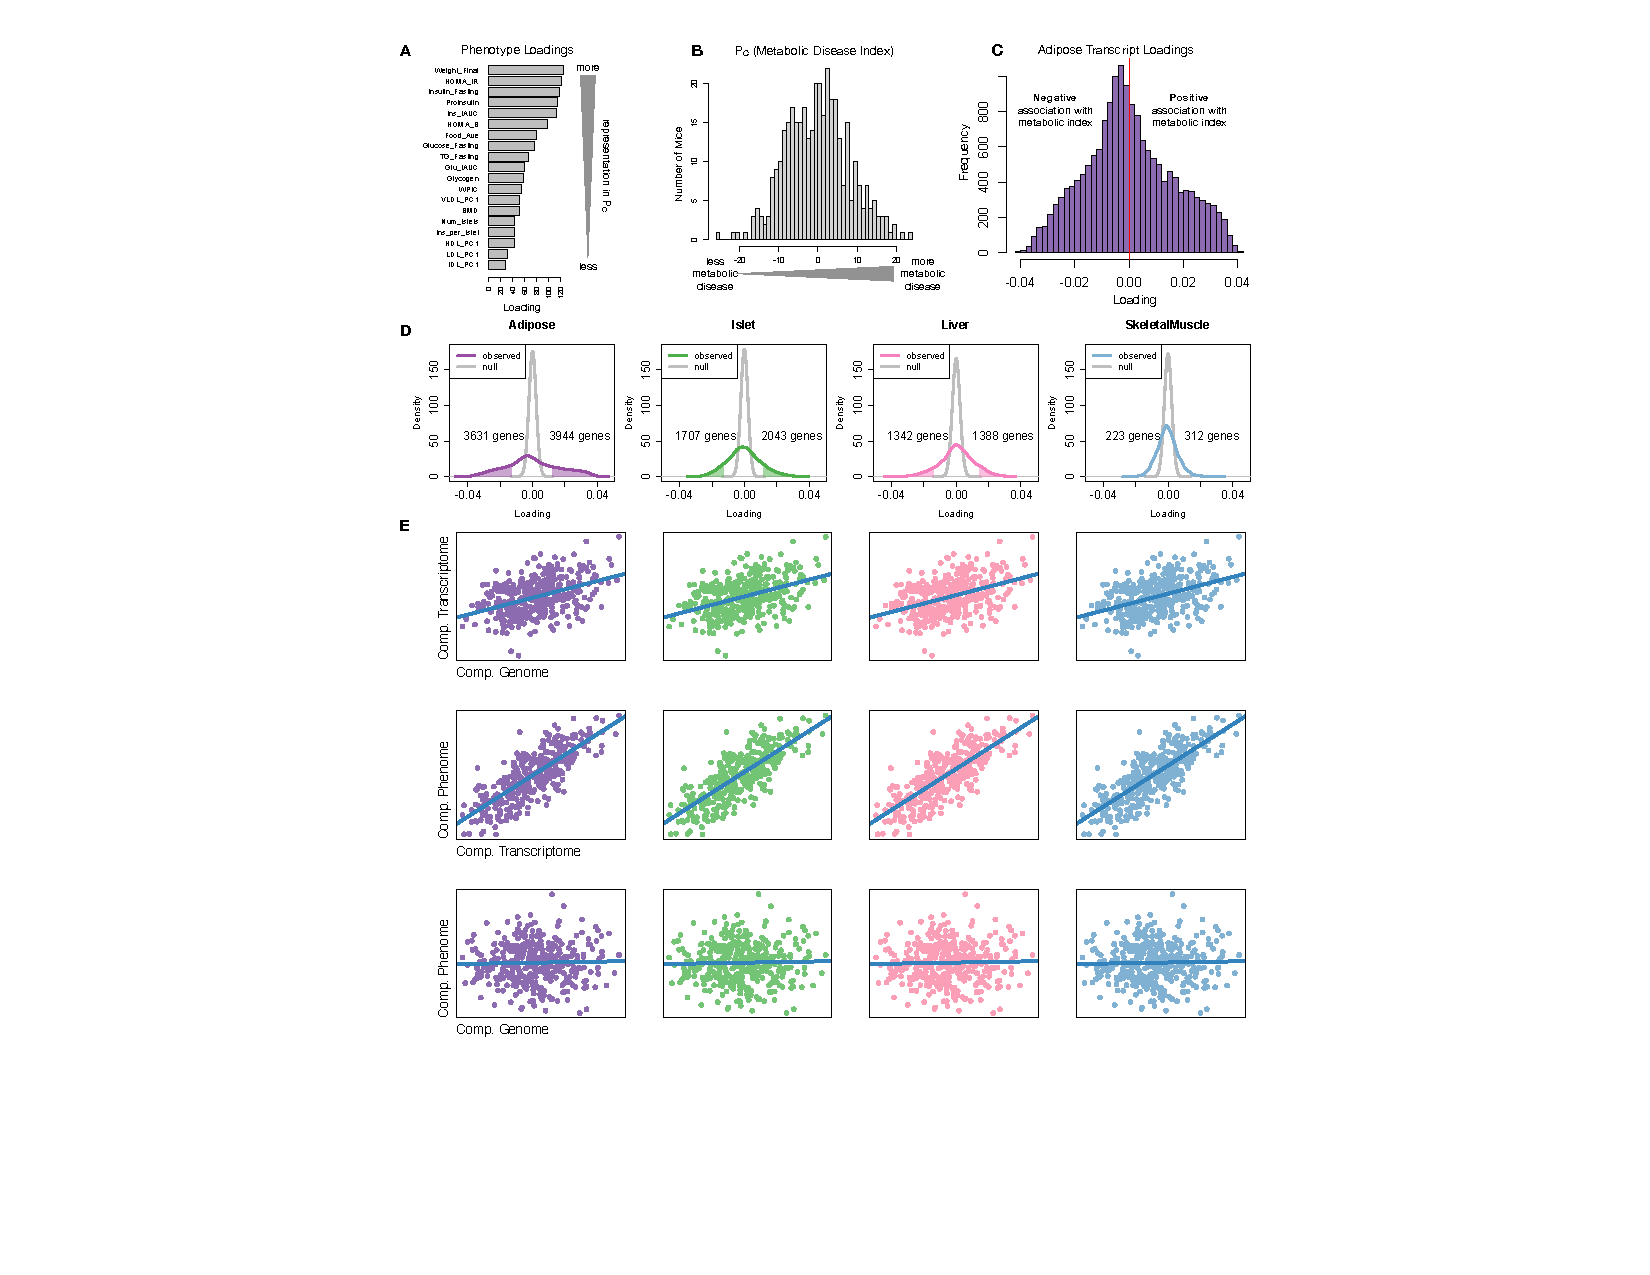
\includegraphics[width=\textwidth]{Figures/Fig4_interpretation.pdf} 
\caption{Interpretation of loadings. \textbf{A.} Loadings 
across traits. Body weight and insulin resistance contributed 
the most to the composite trait. \textbf{B.} Phenotype scores 
across individuals. Individuals with large positive phenotype 
scores had higher body weight and insulin resistance than average. 
Individuals with large negative phenotype scores had lower body 
weight and insulin resistance than average. \textbf{C.} 
Distribution of transcript loadings in adipose tissue. For 
transcripts with large positive loadings, higher expression was 
associated with higher phenotype scores. For transcripts with 
large negative loadings, higher expression was associated with 
lower phenotype scores. \textbf{D.} Distribution of absolute 
value of transcript loadings across tissues. Transcripts in 
adipose tissue had the largest loadings indicating that 
transcripts in adipose tissue were the best mediators of the 
genetic effects on body weight and insulin resistance.
}
\label{fig:interpretation}
\end{figure}

\subsubsection{High-loading transcripts have low local heritability,
high distal heritability, and are linked mechanistically to
obesity}\label{high-loading-transcripts-have-low-local-heritability-high-distal-heritability-and-are-linked-mechanistically-to-obesity}

Transcripts that most strongly correlated with \(T_C\) were the best
mediators of effect of genetics on \(P_C\). Large positive loadings
indicate that inheriting higher expression was associated with a higher
\(P_C\) (higher risk of obesity and metabolic disease on the high-fat
diet) (Fig. \ref{fig:interpretation}C). Conversely, large negative
loadings indicate that inheriting lower expression of these transcripts
was associated with a lower \(P_C\) (lower risk of obesity and metabolic
disease on the high-fat diet) (Fig. \ref{fig:interpretation}C).
Functional enrichments for the most highly correlated and
anti-correlated transcripts are shown in Supp. Fig. \ref{fig:top_enrich}
and represent known biology of obesity and diabetes. In adipose tissue,
for example, the transcripts most strongly correlated with \(T_C\) were
enriched for immune system signaling and cell motility. It is well
established that adipose tissue in obese individuals is highly inflamed
{[}cite{]} and infiltrated by macrophages {[}cite{]}. The transcripts
most strongly negatively correlated with \(T_C\) were enriched for
metabolism of the branched-chain amino acids (BCAA), valine, leuceine,
and isoleucine. BCAA are used in adipose tissue in lipogenesis, and
inhibiting BCAA catabolism inhibits adipogenesis \cite{pmid26571352}.
BCAA levels are also related to insulin resistance and are elevated in
insulin-resistant obese individuals relative to weight-matched
non-insulin reisistand individuals \cite{pmid23512805}. In the DO mice
studied here, inheriting reduced expression of genes involved in BCAA
catabolism was associated with reduced body weight and insulin
resistance.

Transcripts in the adipose tissue had the largest loadings, both
positive and negative, of all tissues, suggesting that much of the
effect of genetics on body weight and insulin reisistance is mediated
through gene expression in adipose tissue (Fig.
\ref{fig:loading_heritability}A). The loadings in liver and pancreas
were comparable, and those in skeletal muscle were the weakest (Fig.
\ref{fig:loading_heritability}A), suggesting that less of the genetic
effects were mediated through transcription in skeletal muscle. Across
all tissues, trahscripts with the largest loadings tended to have
relatively high distal heritability compared with local heritability
(Fig. \ref{fig:loading_heritability}A). Transcripts with the highest
local heritability tended to have very weak loadings and were 3.6 times
less likely to be associated with diabetes and obesity in the literature
than transcripts with high loadings (Fig. fig:loading\_heritabilityB,
Methods). TWAS-nominated transcripts also had relatively weak loadings
and high local heritabilty (Fig. \ref{fig:interpretation}C). They were
half as likely as transcripts with the highest loadings to be associated
with diabetes and obesity in the literature (Fig.
\ref{fig:interpretation}C).

\begin{figure}[ht!]
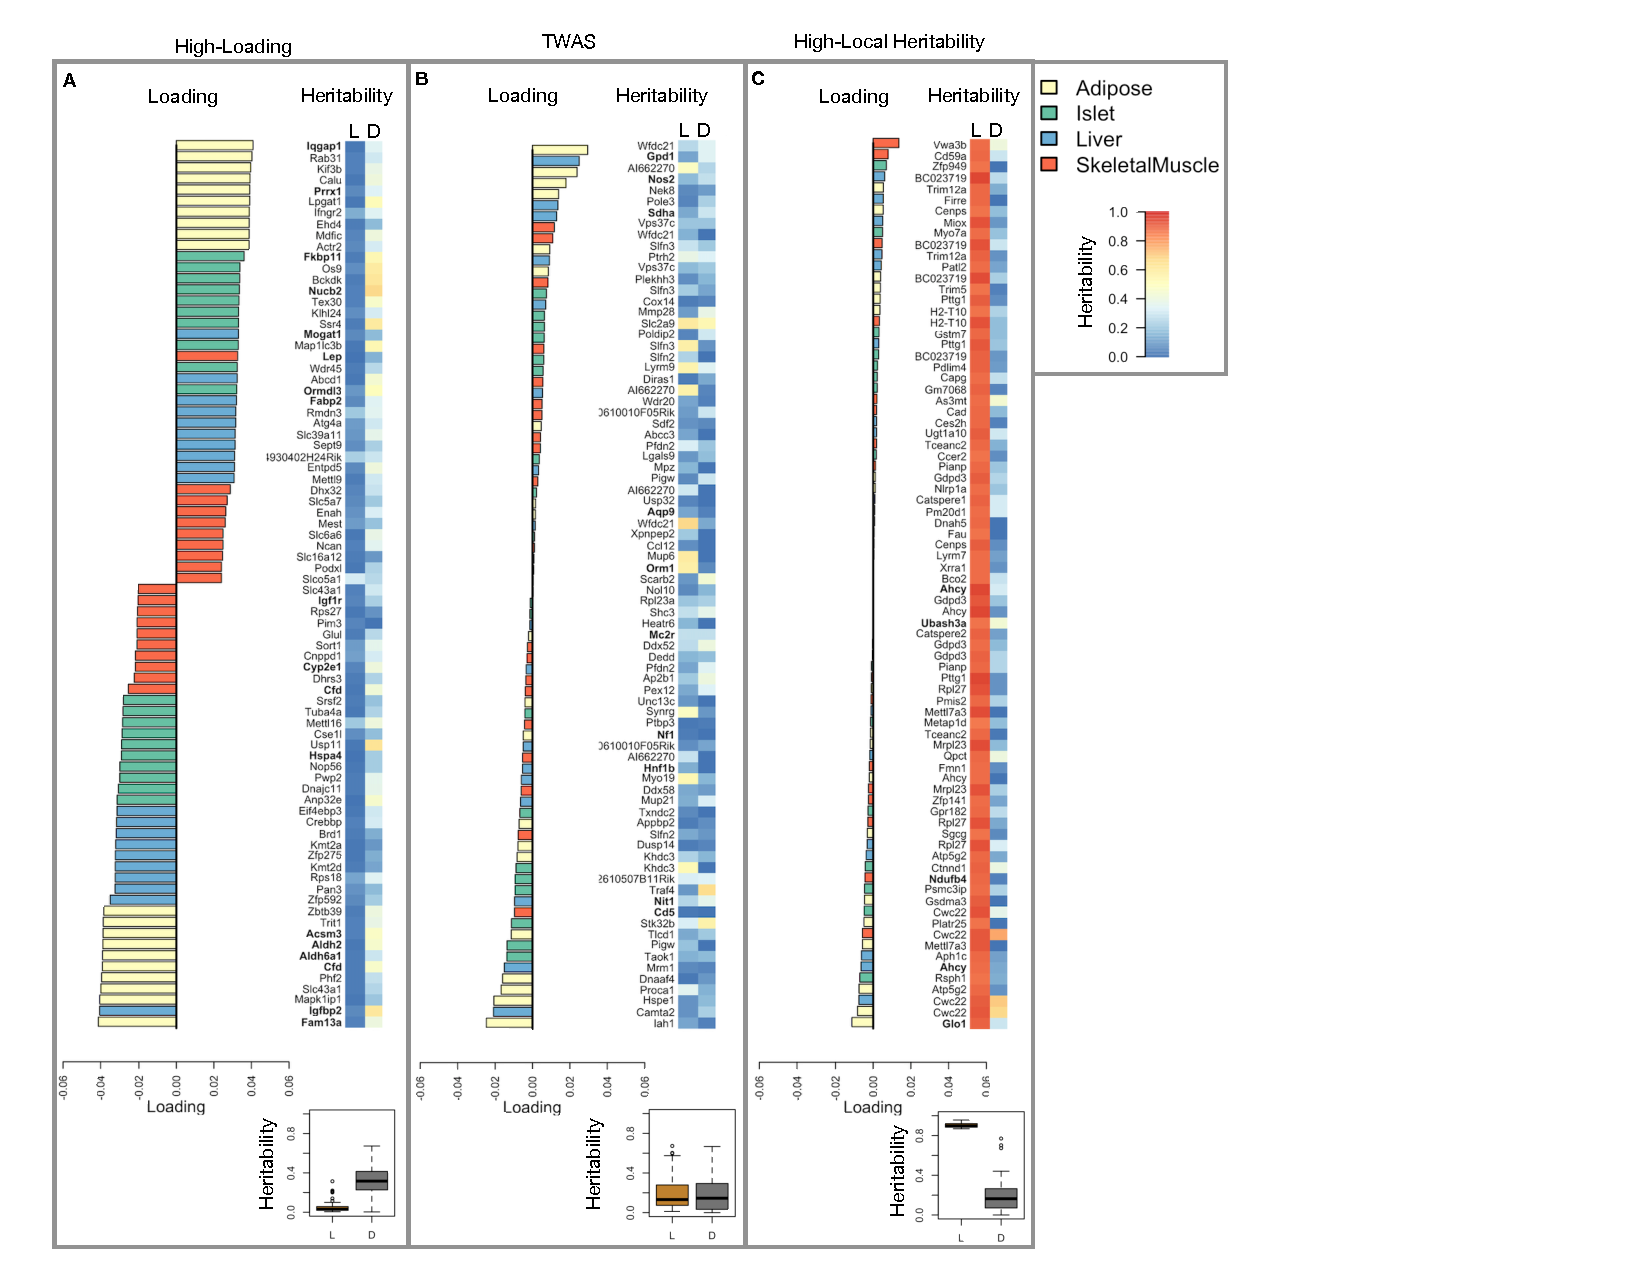
\includegraphics[width=\textwidth]{Figures/Fig5_loading_heritability.pdf} 
\caption{Transcripts with high loadings have high distal heritability
and literature support. Each panel has a bar plot showing the loadings 
of transcripts selected by different criteria. Bar color indicates the 
tissue of origin. The heat map shows the local (L - left) and distal 
(D - right) heritability of each transcript. \textbf{A.} Loadings for 
the 10 transcripts with the largest positive loadings and the 10 
transcripts with the largest negative loadings for each tissue. 
\textbf{B.} Loadings of TWAS candidates with the 10 largest positive 
correlations with traits and the largest negative correlations with 
traits across all four tissues. \textbf{C.} The transcripts with the 
largest local heritability (top 20) across all four tissues.
}
\label{fig:loading_heritability}
\end{figure}

\subsubsection{Tissue-specific transriptional programs are associated
with metabolic
traits}\label{tissue-specific-transriptional-programs-are-associated-with-metabolic-traits}

Clustering of transcripts with top loadings in each tissue shows
tissue-specific functional modules associated with obesity and insuling
resistance in the DO population (Fig. \ref{fig:toa}). Many of these
modules, such as leptin signaling in adipose tissue {[}cite{]} and
skeletal muscle {[}cite{]}, as well as apelin signaling {[}cite{]} have
well established functional roles in diabetes and obesity.

\begin{figure}[ht!]
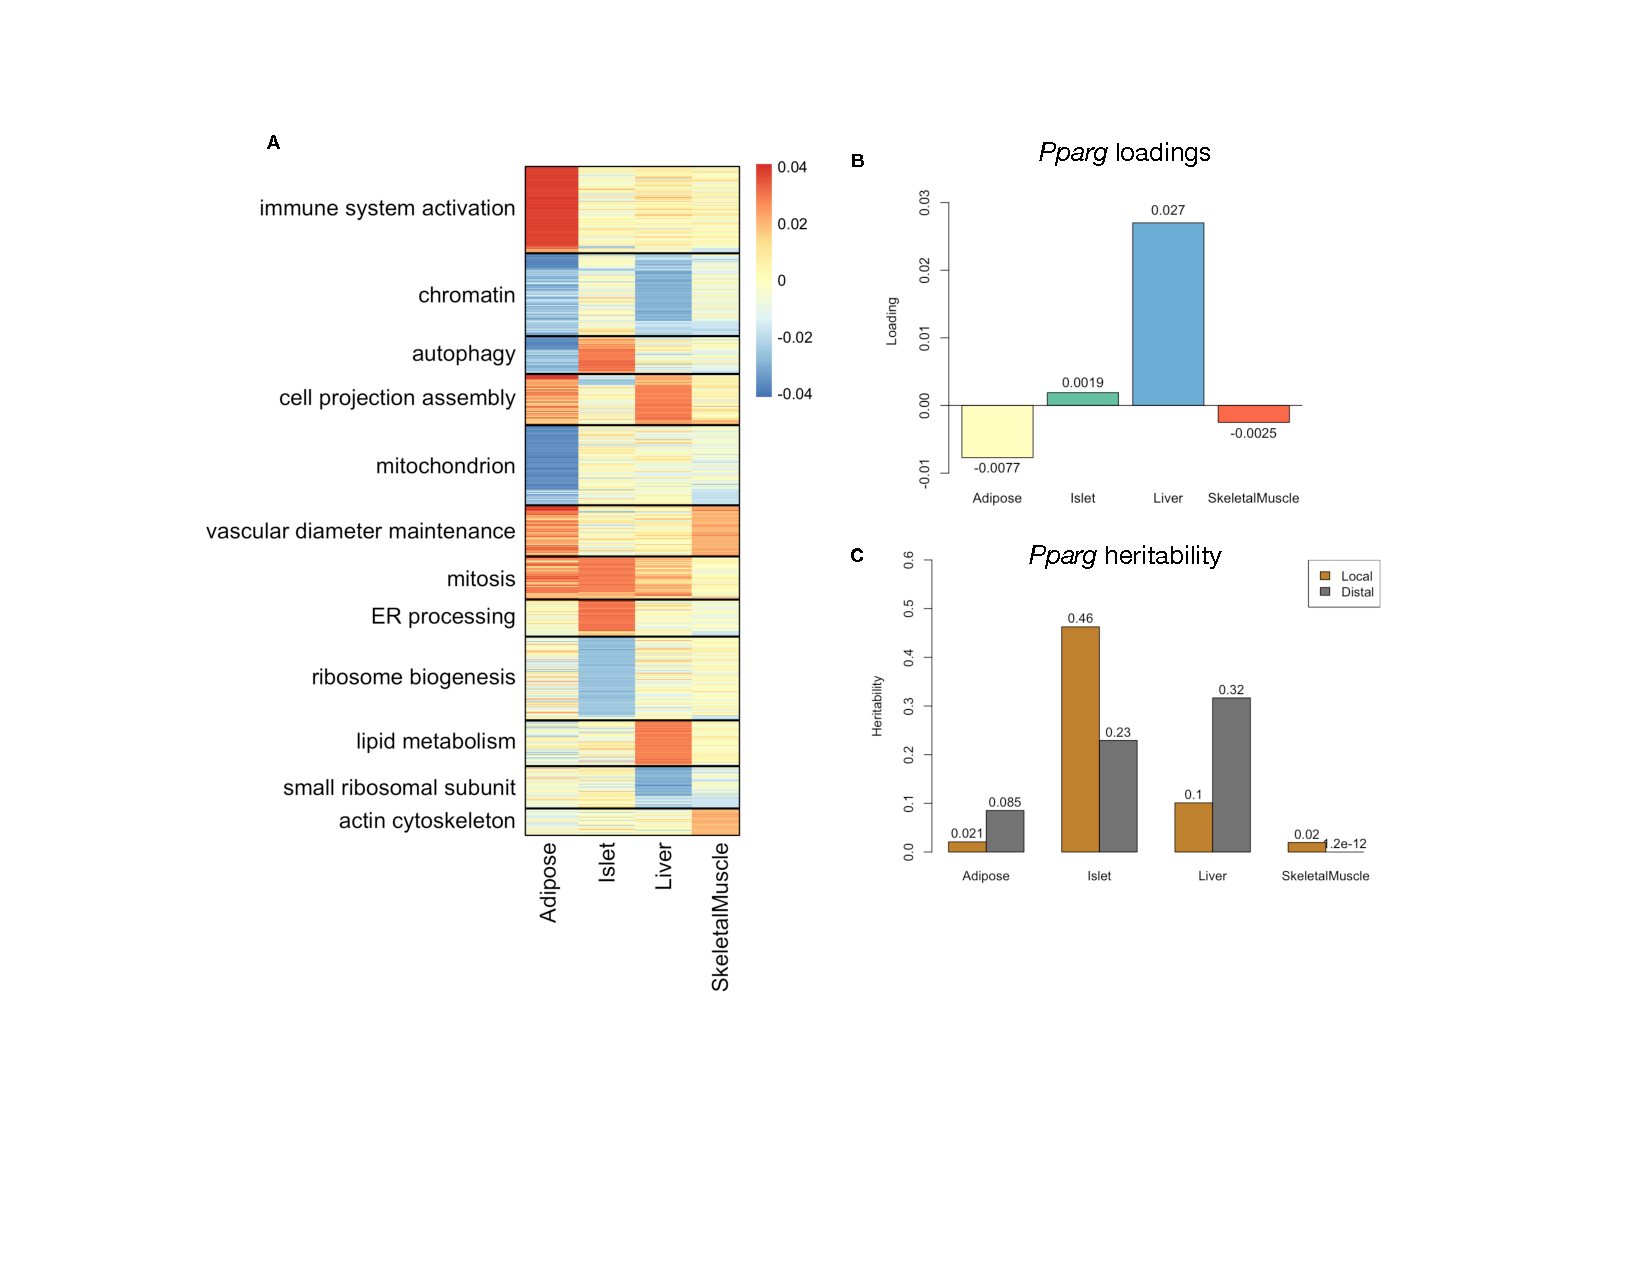
\includegraphics[width=5in]{Figures/Fig6_TOA.pdf} 
\caption{Tissue-specific transcriptional programs are associated 
with obesity and insulin resistance. \textbf{A.} Heat map showing 
the loadings of all transcripts with loadings greater than 2.5 standard 
deviations from the mean in any tissue. The heat map is hierarchically 
clustered. Functional enrichment of each cluster is indicated by color. 
An example cluster enriched for apelin signaling is highlighted. \textbf{B.} 
The distribution of the loadings of the apelin cluster across all tissues. 
These transcripts have positive loadings in the islet, and negative 
loadings in all other tissues. \textbf{C.} Model showing the interactions 
between glucose-stimulated insulin secretion by the pancreas and apelin 
signaling in skeletal and adipose tissue.
}
\label{fig:toa}
\end{figure}

\subsubsection{Gene expression, but not local eQTLs predict body weight
in an independent
population}\label{gene-expression-but-not-local-eqtls-predict-body-weight-in-an-independent-population}

The loading of each transcript indicates how inherited expression levels
influence metabolic phenotypes. If local regulation is the predominant
factor influencing gene expression, we should be able to predict an
individual's phenotype based on their genotypes across all local eQTLs.
We tested this hypothesis in an independent population of F1 mice
generated through multiple pairings of Collaborative Cross (CC)
{[}cite{]} strains (Fig. \ref{fig:cc_prediction}A) (Methods).

\textbackslash begin\{figure\}{[}ht!{]}
\includegraphics[width=\textwidth]{Figures/Fig7_CC_Prediction.pdf}
\textbackslash caption\{Transcription, but not local genotype, predicts
phenotype in the CC-RIX. \textbf{A.} Workflow showing procedure for
translating HDM results to an independent population of mice.
\textbf{B.} Relationships between the predicted metabolic index and
measured body weight. The left column shows the predictions using
measured transcripts. The right column shows the prediction using
transcript levels imputed from local genotype. Gray boxes indicate
measured quantities, and blue boxes indicate calculated quantities. The
dots in each panel represent individual CC-RIX strains. The gray lines
show the standard deviation on body weight for the strain.

\} \label{fig:cc_prediction} \textbackslash end\{figure\}

We first tested whether the transcript loadings derived from HDM in the
DO were relevant to the relationship between the transcriptome and the
phenome in the CC-RIX. To do this, we multiplied the transcript loadings
derived from HDM in the DO mice by transcript measurements in the CC-RIX
standardized across individuals. This created a transcript vector
weighted by importance to metabolic disease as determined in the DO. The
mean of this vector was the predicted metabolic index for the animal
based on its transcription in either adipose tissue, liver, or skeletal
muscle. Across all three tissues, weighted transcription values were
significantly correlated with metabolic index in the CC-RIX population
measured as body weight (Fig. \ref{fig:cc_prediction}B left column).
Adipose tissue transcription yielded the most accurate prediction
(stats). This result confirms the validity and translatability of the
transcript loadings determined in the DO population and their
relationship to metabolic disease. It also supports the observation that
transcription in adipose tissue is the strongest mediator of genetic
effects on metabolic index.

We then tested whether this mediation signal was encoded by local
genotype. To do this, we imputed gene expression in the CC-RIX using
local genotype. We were able to estimate variation in gene transcription
robustly. The correlation between measured gene expression and imputed
gene expression across all tissues was close to \(R = 0.5\), and the
variance explained by local genotype was comparable in the DO and CC-RIX
(Supp. Fig. \ref{fig:cc_imputation}). However, when weighted with the
loadings derived from HDM in the DO population, these imputed
transcripts across all tissues failed to predict metabolic index in the
CC-RIX (Fig. \ref{fig:cc_prediction}B right column).

Taken together, these results support the hypothesis that distal, rather
than local genetic factors are primarily driving complex-trait related
variation in gene expression.

\subsubsection{Distally heritable transcriptomic signatures reflect
variation in composition of adipose tissue and
islets}\label{distally-heritable-transcriptomic-signatures-reflect-variation-in-composition-of-adipose-tissue-and-islets}

Interpretation of global distal genetic influences on gene expression
and phenotype is potentially more challenging than interpretation and
translation of local genetic influences. Effects can not be located to
individual gene variants or transcripts, but because we have a measure
of importance across all transcripts in multiple tissues, we can look at
global patterns. We noted earlier that functional enrichments of
transcripts with large positive loadings in the adipose tissue,
suggested that the obese mice in the population had a genetic
predisposition toward elevated macrophage infiltration into the adipose
tissue. This suggests heritabl variability in cell-type composition of
the adipose tissue. We investigated this further bioinformatically by
comparing the loadings of cell-type-specific transcripts (Methods). For
adipose tissue we used a list of cell-type specific genes identified in
human adipose tissue

In adipose tissue, the mean loading of macrophage-specific genes was
substantially greater than 0 (Fig. \ref{fig:human_translation}A),
indicating that obese mice were genetically predisposed to have high
levels of macrophage infiltration in adipose tissue in response to the
high-fat, high-sugar diet.

\begin{figure}[ht!]
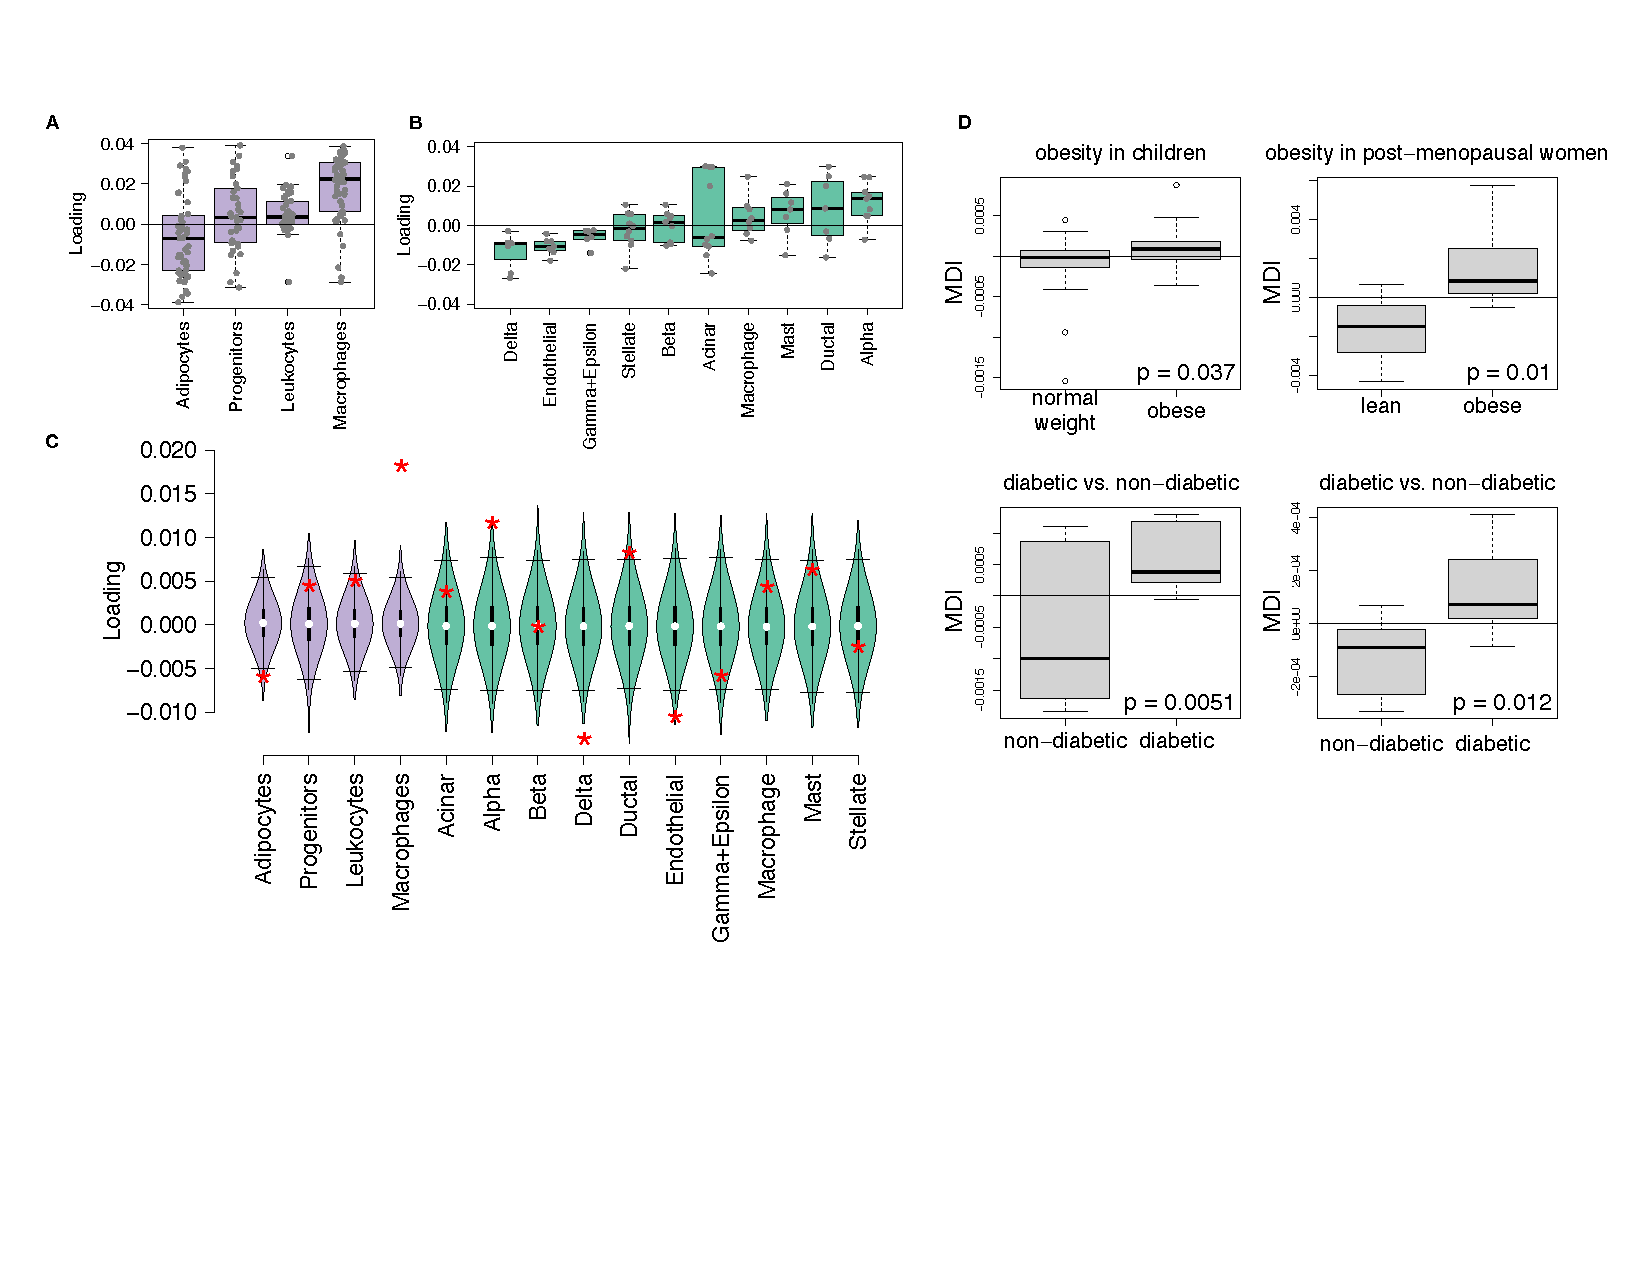
\includegraphics[width=\textwidth]{Figures/Fig8_Human_Translation.pdf} 
\caption{HDM results translate to humans. \textbf{A.} Distribution of 
loadings for cell-type-specific transcripts in adipose tissue. \textbf{B.} 
Distribution of loadings for cell-type-specific transcripts in pancreatic 
islets (green). \textbf{C.} Null distributions for the mean loading of 
randomly selected transcripts in each cell type compared with the observed 
mean loading of each group of transcripts (red asterisk). \textbf{D.} 
Predictions of metabolic phenotypes in four adipose transcription data 
sets downloaded from GEO. In each study the obese/diabetic patients were 
predicted to have greater metabolic disease than the lean/non-diabetic 
patients based on the HDM results from DO mice.
}
\label{fig:human_translation}
\end{figure}

In islet, the mean loadings for alpha-cell specific transcripts were
significantly positive, while the mean loadings for delta- and
endothelial-cell specific genes were significantly negative (Fig.
\ref{fig:human_translation}B). These results suggest that obese mice had
inherited higher proportions of alpha cells, and lower proportions of
endothelial and delta cells in their pancreatic islets.

The loadings for pancreatic beta cell-type specific loadings was not
significantly different from zero. This does not reflect on the function
of the beta cells in the obese mice, but rather suggests that mice prone
to obesity were not obese because they inherited fewer beta cells than
non-obese mice.

Biological interpretation of alpha, endothelial, delta cells??

\subsubsection{Distally heritable transcriptomic signatures translate to
human
disease}\label{distally-heritable-transcriptomic-signatures-translate-to-human-disease}

Ultimately, the distally heritable transcriptomic signatures that we
identified in DO mice will be useful if they inform pathogenicity and
treatment of human disease. To investigate the potential for translation
of the gene signatures identified in DO mice, we compared them to
transcriptional profiles in obese and non-obese human subjects
(Methods). We limited our analysis to adipose tissue because the adipose
tissue signature had the strongest relationship to obesity and insulin
resistance in the DO.

We calculated a predicted obesity score for each individual in the human
studies based on their adipose tissue gene expression (Methods) and
compared the predicted scores for obese and non-obese groups as well as
diabetic and non-diabetic groups. In all cases, the predicted obesity
scores were higher on average for individuals in the obese and diabetic
groups compared with the lean and non-diabetic groups, indicating that
the distally heritable signature of obesity identified in DO mice is
relevant to obesity and diabetes in human subjects.

\subsubsection{Targeting gene
signatures}\label{targeting-gene-signatures}

Although high-loading transcripts are likely good candidates for
understanding specific biology related to obesity, we emphasize that the
transcriptome overall is highly interconnected and redundant, and that
focusing on individual transcripts for treatment may be less effective
than using the transcriptomic signature as a whole. The ConnectivityMap
(CMAP) database {[}cite{]} developed by the Broad Institute allows us to
query thousands of compounds that reverse or enhance transcriptomic
signatures as a whole in multiple different cell types. By identifying
drugs that reverse pathogenic transcriptomic signatures as a whole
rather than targeting individual genes, we can potentially increase
efficacy of tested compounds.

We thus queried the CMAP database through the CLUE online query tool
developed by The Broad Institute {[}cite{]} (Methods).

Alternatively, we can target the gene signature as a whole using CMAP.
Identifying drugs to target gene signatures is possible through CMAP. We
put our loadings from islet into CMAP. The top hit was PPAR receptor
agonist. Rosiglitazone, a widely used diabetes drug, is a PPAR receptor
agonist. Another class of drugs on the list was sufonylureas, which are
another major class of drugs for type 2 diabetes.

\begin{itemize}
\tightlist
\item
  \textbf{Supplemental Table} results from CMAP
\end{itemize}

\subsection{Discussion}\label{discussion}

\begin{itemize}
\tightlist
\item
  distal heritability correlates with phenotype relevance
\end{itemize}

\subsection{Data Availability}\label{data-availability}

Here we tell people where to find the data

\subsection{Acknowledgements}\label{acknowledgements}

Here we thank people

\pagebreak

\subsection{Supplemental Figures}\label{supplemental-figures}

\begin{figure}[ht!]
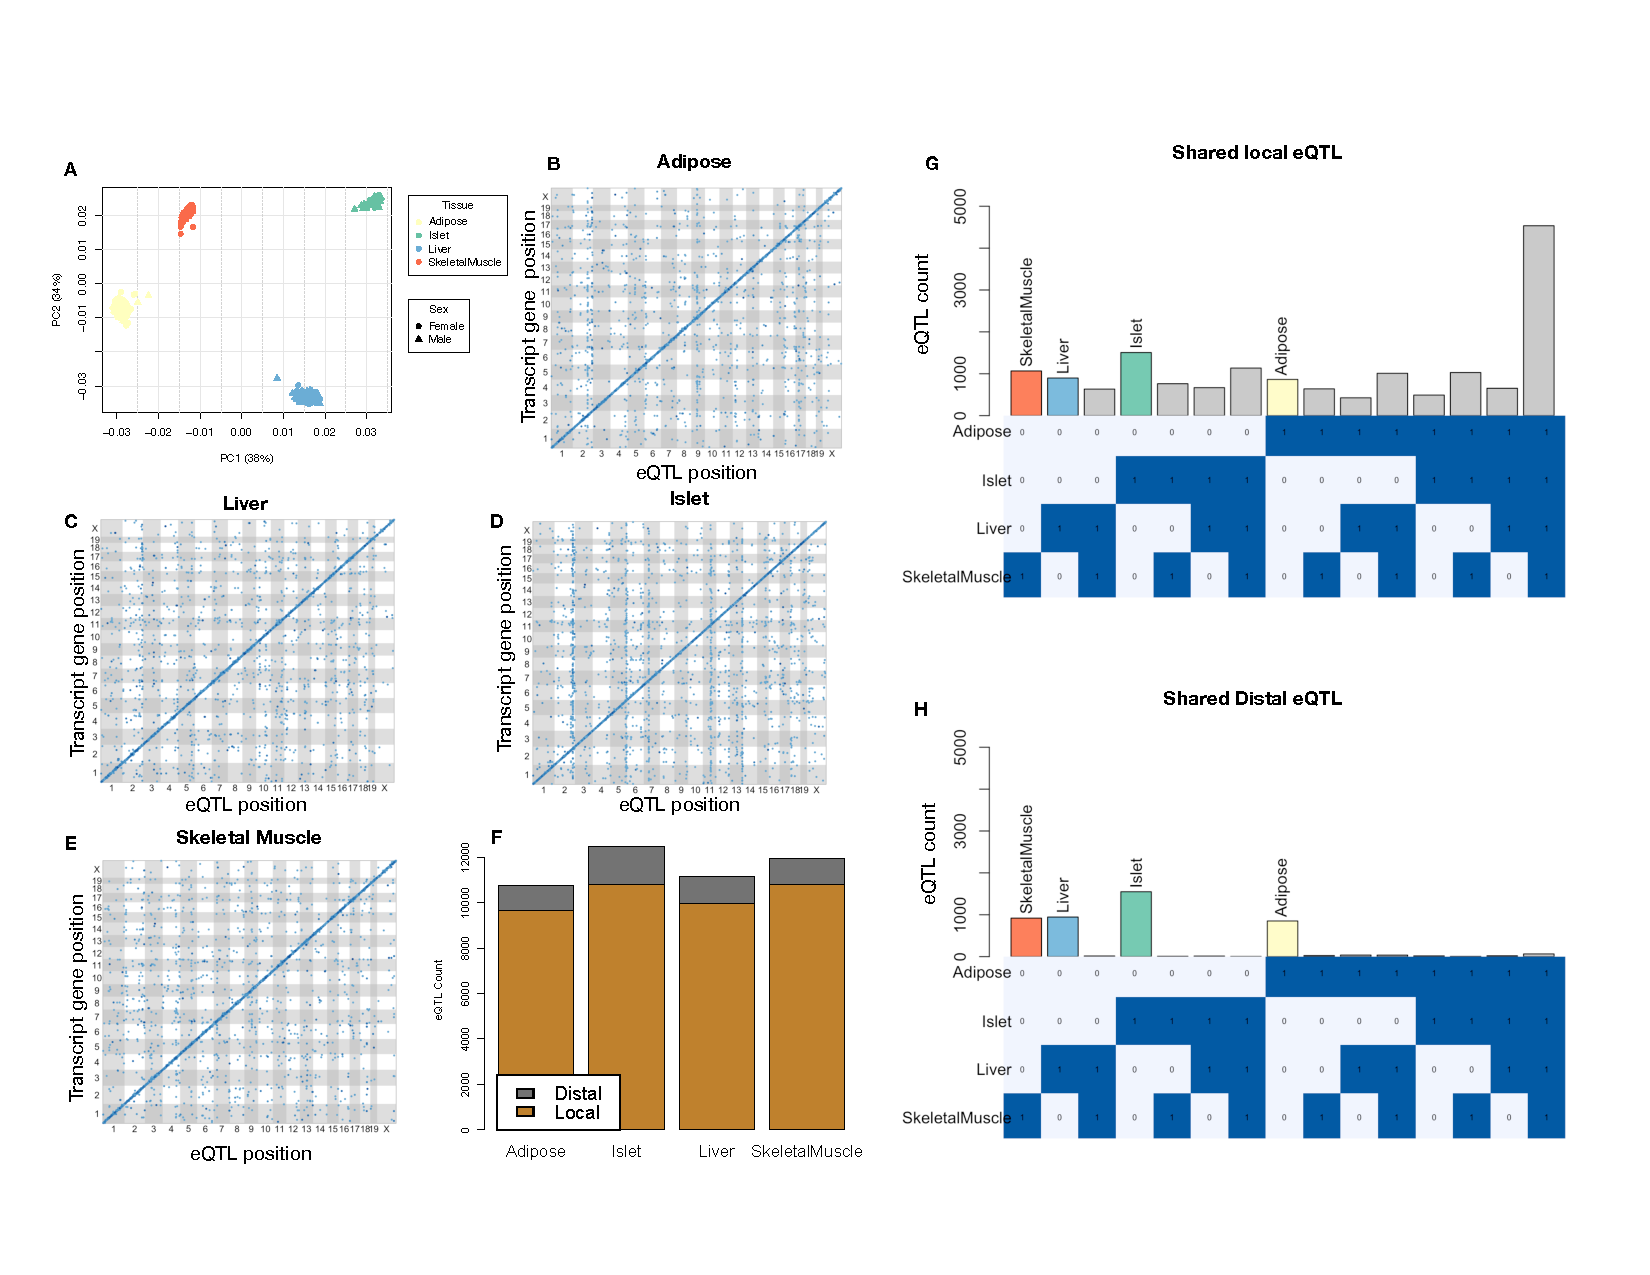
\includegraphics[width=\textwidth]{Figures/Supp_Fig1_eQTL.pdf} 
\caption{Overview of eQTL analysis in DO mice. \textbf{A.} RNA seq 
samples from the four different tissues clustered by tissue. 
\textbf{B.-E.} eQTL maps are shown for each tissue. The $x$-axis 
shows the position of the mapped eQTL, and the $y$-axis shows the 
physical position of the gene encoding each mapped transcript. 
Each dot represents an eQTL with a minimum LOD score of 8. The dots 
on the diagonal are locally regulated eQTL for which the mapped eQTL 
is at the within 4Mb of the encoding gene. Dots off the diagonal are 
distally regulated eQTL for which the mapped eQTL is distant from the 
gene encoding the transcript. \textbf{F.} Comparison of the total number 
of local and distal eQTL with a minimum LOD score of 8 in each tissue. 
All tissues have comparable numbers of eQTL. Local eQTL are much more 
numerous than distal eQTL. \textbf{G.} Counts of transcripts with local 
eQTL shared across multiple tissues. The majority of local eQTL were 
shared across all four tissues. \textbf{H.} Counts of transcripts with 
distal eQTL shared across multiple tissues. The majority of distal eQTL 
were tissue-specific and not shared across multiple tissues. For both G 
and H, eQTL for a given transcript were considered shared in two tissues 
if they were within 4Mb of each other. Colored bars indicate the counts 
for individual tissues for easy of visualization.
}
\label{fig:eQTL}
\end{figure}

\begin{figure}[ht!]
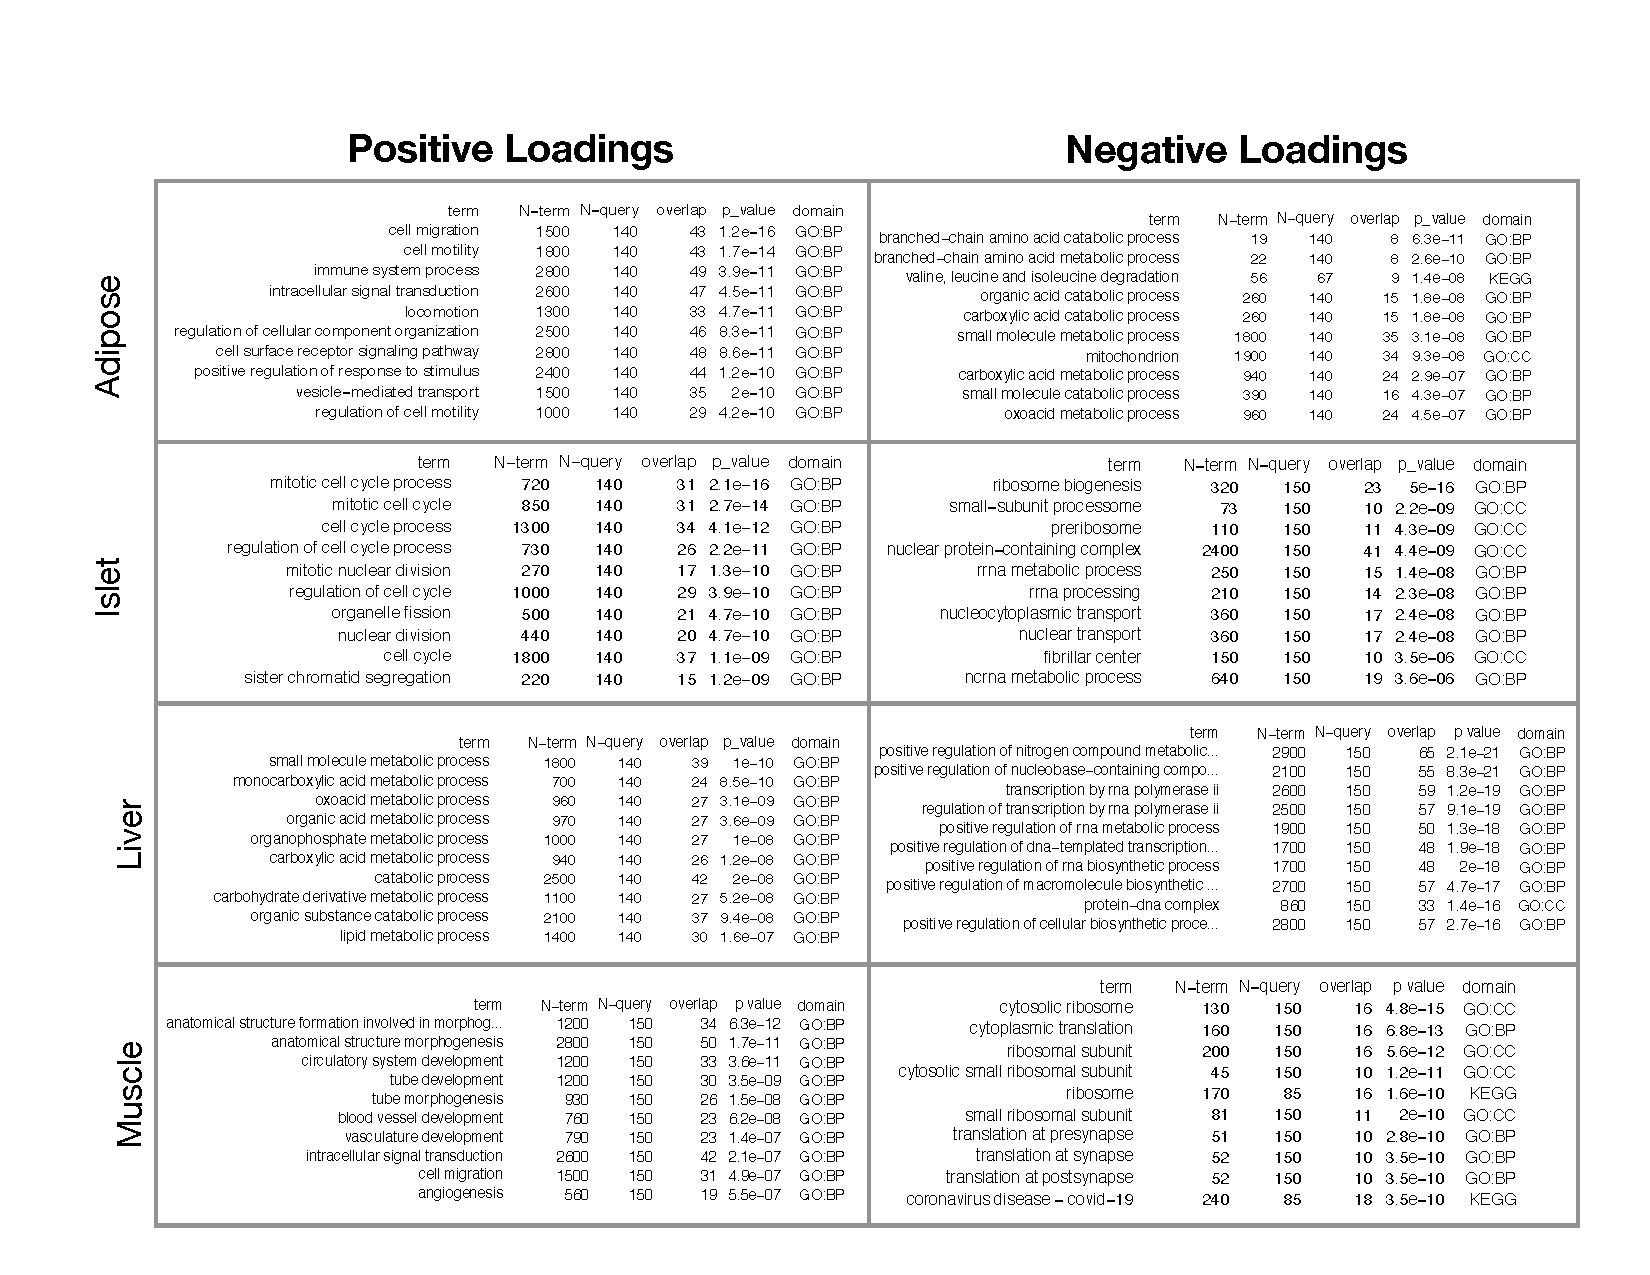
\includegraphics[width=\textwidth]{Figures/Supp_Fig_enrichments.pdf} 
\caption{Tables showing top 10 functional enrichments for 
the 150 transcripts with the largest positive and negative 
loadings across all four tissues.
}
\label{fig:top_enrich}
\end{figure}

\begin{figure}[ht!]
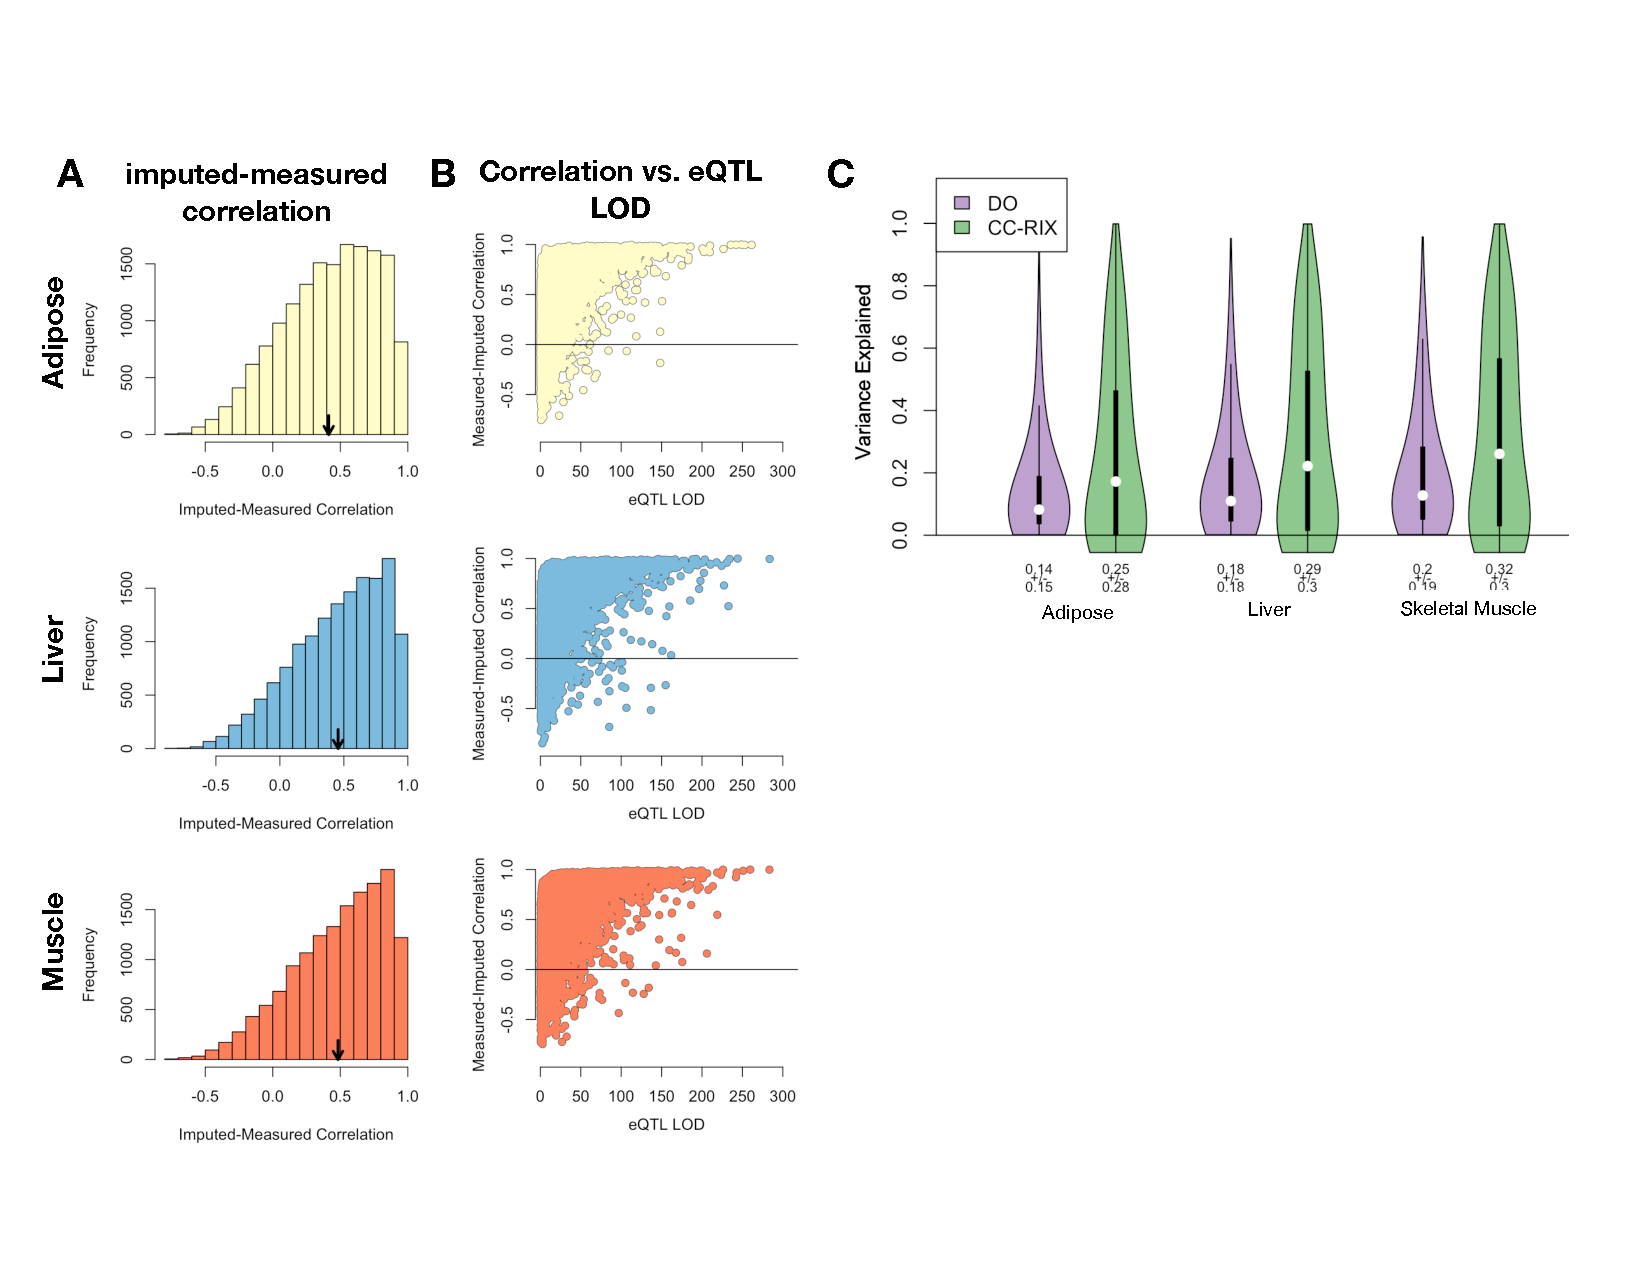
\includegraphics[width=\textwidth]{Figures/Supp_Fig_CC-RIX_Imputation.pdf} 
\caption{Validation of transcript imputation in the CC-RIX. \textbf{A.} 
Distributions of correlations between imputed and measured transcripts 
in the CC-RIX. The mean of each distribution is shown by the red line. 
All distributions were skewed toward positive correlations and had
 positive means near a Pearson correlation (r) of 0.5. \textbf{B.} 
 The relationship between the correlation between measured and 
 imputed expression in the CC-RIX (x-axis) and eQTL LOD score. As 
 expected, imputations are more accurate for transcripts with strong 
 local eQTL. \textbf{C.} Variance explained by local genotype in the 
 DO and CC-RIX. 
}
\label{fig:cc_imputation}
\end{figure}

\pagebreak

\bibliographystyle{unsrt}
\bibliography{islet.bib}

\end{document}
